\section{Theorie}
\label{sec:Theorie}

Ein Lock-In-Verstärker wird benutzt, um (stark) verrauschte periodische Signale zu verstärken und zu messen. Dazu wird das Signal, welches zuvor durch einen Bandpassfilter von höher- ($\omega \gg \omega_0$) und niederfrequentem ($\omega \ll \omega_0$) Rauschen befreit wurde mit einem Referenzsignal moduliert. Dieses kann durch einen Phasenschieber an das zu messende Signal angeglichen werden, sodass die Schwinugen in Phase sind ($\Delta \phi = 0$). Zuletzt wird das Mischsignal mit einem Tiefpassfilter über mehrere Perioden aufintegriert, wobei sich die stochastischen Rauschanteile bei ausreichender Zeitkonstante $\tau = RC \gg \sfrac{1}{\omega_0}$ aufheben.

\begin{figure}
  \centering
  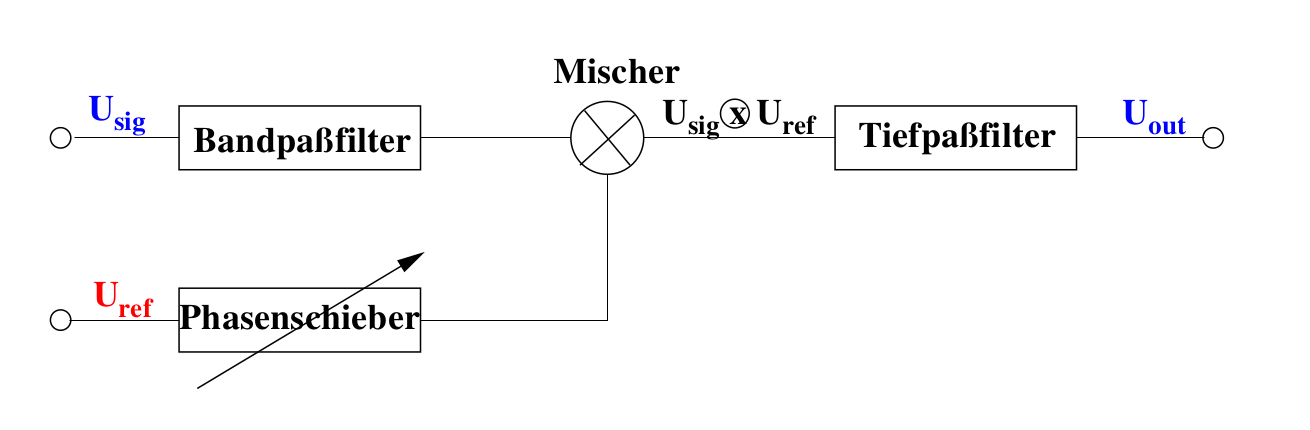
\includegraphics[width=\textwidth]{content/grafiken/Schema.png}
  \caption{Schematische Darstellung eines Lock-In-Verstärkers}
  \label{fig:schema}
\end{figure}

\begin{figure}
  \centering
  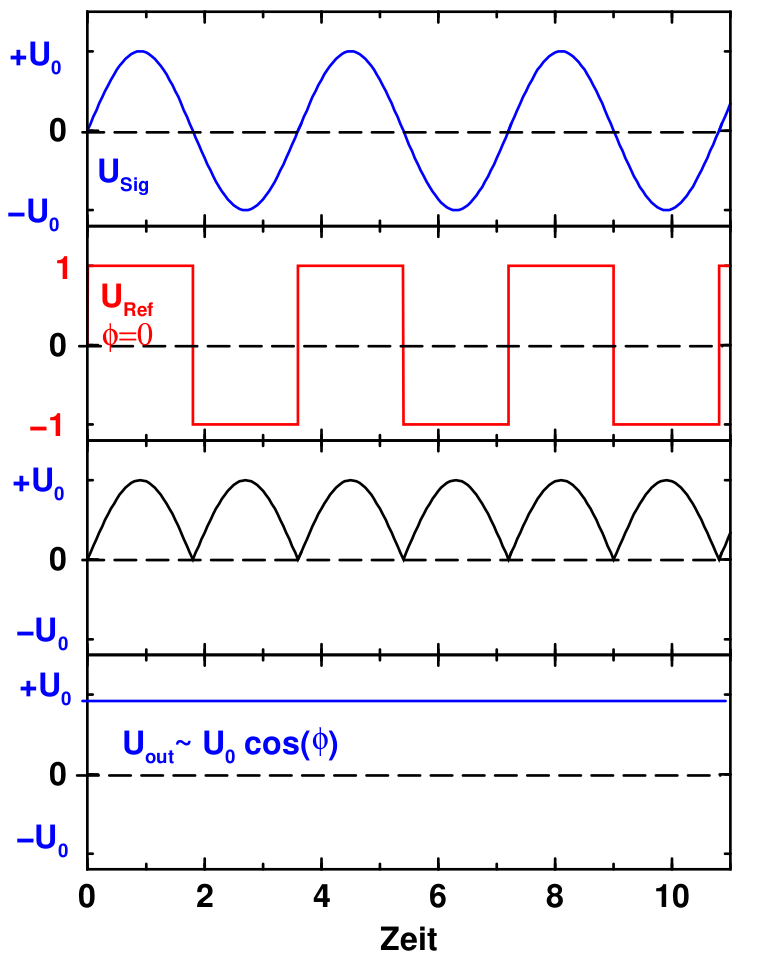
\includegraphics[width=.5\textwidth]{content/grafiken/Wellen.png}
  \caption{Schematische Darstellung eines Lock-In-Verstärkers}
  \label{fig:wellen}
\end{figure}

Für eine sinusförmige Spannung
\begin{equation}
  U_\mathrm{sig} = U_0 \cdot \sin (\omega t),
\end{equation}
welche mit einer synchronisierten Rechteckspannung $U_\mathrm{ref}$ der Amplitude $1$ moduliert wird, ergibt sich, wie in Abb.~\ref{fig:wellen} ersichtlich nach der Modulation ein Signal welches dem Betrag der Signalspannung entspricht. Die unteren Halbwellen wurden also an der Zeitachse gespiegelt.
Zur Bestimmung der Ausgangsspannung wird nun das Referenzsignal mit einer Fourier-Reihe genähert, sodass
\begin{equation}
  U_\mathrm{ref} = \frac{4}{\pi} \left( \sin(\omega t) + \frac{1}{3} \sin(3\omega t) + \frac{1}{5} \sin(5\omega t) + … \right)
\end{equation}
ist. Das Produkt des Signals mit der Referenzschwingung, also das modulierte Signal hat somit die Schwingungsgleichung
\begin{equation}
  U_\mathrm{sig} \times U_\mathrm{ref} = \frac{2}{\pi} U_0 \left( 1 - \frac{2}{3} \sin(2 \omega t) + \frac{2}{15} \sin(4\omega t) + \frac{2}{35} \sin(6\omega t) + … \right).
\end{equation}
Durch den Tiefpassfilter werden zuletzt die Schwingungsanteile entfernt und übrig bleibt nur die Ausgangsspannung
\begin{equation}
  U_\mathrm{out} = \frac{2}{\pi} U_0.
\end{equation}
Sind $U_\mathrm{ref}$ und $U_\mathrm{sig}$ nicht in Phase, sondern mit einer Phasenschiebung $\phi$ versehen, ist die Ausgangsspannung von dieser abhängig:
\begin{equation}
  \label{eqn:ganzwichtig}
  U_\mathrm{out} = \frac{2}{\pi} U_0 \cos \phi
\end{equation}
